\documentclass[10pt,conference]{IEEEtran}
\let\labelindent\relax
\usepackage{cite}
\usepackage{enumitem}
\usepackage{graphicx}
\usepackage{subcaption}
\usepackage{url}

\title{Title}
\author{\IEEEauthorblockN{Chelsea Farley, Ryan Lewis, David Armstrong, Rina Gao and Ryunosuke Madenokoji}
\IEEEauthorblockA{The University of Auckland}}
\date{Today}

\begin{document}
\maketitle

\begin{abstract}
The overall traffic volume on the Web is continually growing as is user expectations, which has highlighted the need to optimise the performance of the Web. In this paper we will analyse two Web server logs from 1994-1995 and one from 2006-2007. This paper will focus on characterising the workload based on success rates, document types, concentration of references, one time referencing, file size distribution, usage patterns and caching. An emphasis will be placed on how the characteristics of the workloads have changed over time, and as such we have identified several changes in workload characteristics. Finally, the knowledge gained from this study will be linked to practical implications and areas which could benefit from optimisations.
\end{abstract}

\section{Introduction}
There has been an increase in the overall traffic volume on the Web. The rate of increase of data traffic has been shown to follow Moore's law \cite{williams05}. Moore's law as it pertains to data traffic, states that the overall traffic volume will double annually. This property of data traffic means that the scalability of the Web is more important than ever. Additionally, the time an average user will wait for a page to load has decreased from eight seconds in 2000 to three seconds in 2009 \cite{Butkiewicz}. Therefore, it is becoming paramount that optimisations are made to improve Web performance.

In order to improve the performance and scalability of the Web, we must first develop an understanding of current Web workload characteristics and how they have changed over time. An understanding of the evolution of workload characteristics is vital in the development of effective caching architectures which, in turn, leads to improved performance. Additionally, workload analysis can aid in capacity planning, generating workload-generating models and network administration. Therefore, the purpose of this paper is to revisit several of the invariants identified by Arlitt and Williamson \cite{keynote} and evaluate whether they are applicable to a more recent Web server log. We will be analysing two of the Web server logs used in Arlitt and Williamson's original study: a departmental-level Web server at the University of Calgary and a campus-wide Web server at the University of Saskatchewan \cite{keynote}. Our more recent Web server log has data that was collected over a one year period between 2006 and 2007 from an academic conference Web site.

The remainder of the paper is organised as follows. In the following section we will discuss works related to our analysis and what our investigation contributes. In section \ref{methodology} we describe the characteristics we have chosen to analyse, and the metrics and tools we used to perform this study. Then we will explain the results we recorded in section \ref{results} and explain the practical implications of these results in section \ref{discussion}. Finally, we will conclude our paper and examine potential future work in the area of web workload characterisation in section \ref{conclusions}.

\section{Related Work}\label{related_work}
There have been several studies investigating the characteristics of Web workloads. These studies can be useful in understanding the evolution of Web traffic under differing conditions. In order to improve the scalability and performance of the Internet, we must have a complete understanding of the different traffic flows it may have to withstand. We have summarised several previous studies to provide an overview of these traffic flows. 

Arlitt and Jin \cite{world_cup} analysed data from the 1994 World Cup website. This study was motivated by the high volume of users accessing the site, and therefore the potential to extrapolate the future characteristics of web traffic. They discovered that most users are interested in cacheable files and thus caching plays an important role in the scalability and performance of the Internet. They also found that most user sessions had only one request per session, and therefore managing how connections are closed may be improved by examining session properties.

In 1996 and 1997, Arlitt and Williamson \cite{keynote, invariants} analysed logs from six Web servers and presented their findings. The motivation of their study was to find invariants of Web workload characteristics across six server logs. These invariants would be useful in the development of techniques for improving caching and the general performance of the Web. They found 10 invariants which may be useful in future analyses of Web traffic. They also discovered that there is the opportunity for caching to improve performance, and more specifically that caching to reduce the number of requests may be more effective than caching to reduce bytes transferred. 
This study was superseded by a study by Faber et al. \cite{Faber} which looked into the original ten invariants, but also discovered three more. Their study concludes that many of the original ten invariants have remained relatively the same in the twenty years that have passed. Among the three new invariants discovered, one showed a significant difference in results between scientific and general websites.

Williams et al. \cite{williams05} produced an analysis of Web server logs from 2004 from the same three universities as the initial paper \cite{keynote}. The aim of the analysis was to uncover the impact of Moore's law on the ten invariants of the initial study. They concluded that despite the increase in traffic volume, most of the ten invariants remained unchanged. However, the percentage of successful requests and the percentage of HTML and image files transferred had decreased. 

In 2007, Gill et al. \cite{youtube} analysed YouTube usage on the University of Calgary network and collected statistics on global video popularity. The aim of this study was to investigate Web 2.0 workload characteristics to allow for improvements in network management, capacity planning and the design of new systems. Web 2.0 marks a shift towards user generated content and with it comes a plethora of metadata. It was found that although the concentration of references was reduced from that of traditional Web workloads \cite{keynote}, metadata should be used to improve the effectiveness of caching.

Cherkasova and Gupta \cite{Cherkasova} investigated client access patterns, media server access trends, and the evolution of media on websites over time. Their research was split into static and temporal analysis of the data. They looked at the locality of accesses, which was similar to that of a Web server with 14\%-30\% of the server files accounting for 90\% of media sessions, and 92\%-94\% of the bytes transferred. Additionally, 16\%-19\% of files were accessed only once, and the first five weeks of a file’s existence account for 70\%-80\% of its total accesses. They also looked into the trends associated with media session lengths, and the behavior of clients with incomplete sessions. Their research concentrated on comparing media server workloads with traditional web server workloads.

In 2002, Bai and Williamson \cite{Bai} analysed the request arrival rate at each level of a multi-layer web proxy caching hierarchy using trace-driven simulation and artificial web workloads. The presence of a Web proxy cache means that requests are removed from the Web server request stream when there is a cache hit at the proxy. The results showed that there was a decrease in the peak and mean request arrival rates in the presence of a multi-layer web caching hierarchy. However, they also noted that the burstiness of request arrivals may vary or stay the same. They discovered that a gamma distribution may be used to model the arrival of requests in a web caching hierarchy.

Almeida et al. \cite{almeida} analysed the performance of a PC acting as dedicated Web server. The purpose of their study was to measure the activity and resource consumption of the operating system using WebMonitor. This provided insight into variances in the performance of servicing web requests. They observed similar user session properties to Arlitt and Jin \cite{world_cup} as most requests required a new connection, which may be problematic for operating systems that are not designed to cope with this. This highlighted the importance of operating system and network protocol implementation.

Almeida et al. \cite{reference_locality} examined models for gathering data on spatial and temporal locality. The motivation of this study was the insufficiency of simple popularity based models being insufficient for capturing spatial and temporal locality. They discovered that for accesses following a temporal access pattern, caching is beneficial in improving performance. Whereas, for accesses following a spatial access pattern, prefetching is beneficial in improving performance.

In 2012, Tantithamthavorn and Rungsawang \cite{facebook} conducted a study on Facebook usage at Kasetsart University based on a Web traffic log. Their study analysed the time spent communicating online, distribution of HTTP requests, Facebook traffic workload analysis, and more. The results showed that the distribution of HTTP Requests at the level of hostname followed a Zipfian distribution. Additionally, they suggested that long running sessions may be due to idle users. Overall the study showed a typical Web workload at a university.

This paper aims to further contribute to the understanding of workload characteristics and examine how they are applicable to practical situations. In particular, we will examine potential areas where caching could be optimised to provide better performance.

\section{Methodology}\label{methodology}
\subsection{Characteristics}\label{lab:characteristics}
In this study, we have chosen to examine five of the characteristics identified by Arlitt and Williamson \cite{keynote}: the success rate, file types, file size distribution, one time referencing, and the concentration of references. We also look into two of the invariants found by Faber et al. \cite{Faber}: weekday versus weekend usage and diurnal usage. Finally, we add two original invariants: cache hit rate, and the effectiveness of caching.

The success rate looks at the occurrence of successful, found, and not modified status codes of requests to each of the three web servers. Size distribution examines the trend in the sizes of files across each of the three data sets. One time referencing looks at the percentage of files and bytes that are requested only once in the logged period, while the concentration of references is a measurement of the frequency of distinct file accesses. We compare the usage of these sites during weekdays and weekends, and also during daytime and nighttime.
Cache hit rate looks at the ratio of number of accesses to a file compared to the number of times it was cached. While the effectiveness of caching refers to the amount of bandwidth saved with caching.

\subsection{Metrics}
To determine which characteristics from section \ref{lab:characteristics} were present we decided on the following metrics:
\begin{itemize}[noitemsep]
    \item Number of times each status code appears
    \item Number of times each file is accessed
    \item Size of each file transferred
    \item Total number of bytes transferred
    \item The time each file is accessed
\end{itemize}

\subsubsection{Number of times each status code appears}
We recorded a count of each status code or range of status codes so that we could characterise both success rate and caching.
The number of successful requests is the total number of requests that had the status code of either 2xx (Success) or 3xx (Redirection). This allows us to characterise the workloads based on percentage of successful requests.
We also were able to see how many requests were cached by the client based on the count of 304 (Not Modified) status codes in the logs. Counting the number of 304 statuses compared to the total number of requests allows us to characterize the effectiveness of caching.

\subsubsection{Number of times each file is accessed}
This metric is a count of each access to a particular resource.
The measurements produced by this metric show how concentrated the requests are in terms of which files are the most popular and would benefit from higher availablility. In addition this metric will show the number of files accessed only once.

\subsubsection{Size of each file transferred}
This metric gathers the size of each file that is transferred. We used it to calculate the mean and median size for each request. 
It also allowed us to calculate the bandwidth savings from client side caching by combining this metric with the status codes collected.

\subsubsection{Total number of bytes transferred}
This metric simply totalled up the total bandwidth used over the logging period. It allowed us to see the relative effect of caching when comparing the two datasets of different sizes.

\subsubsection{The time each file is accessed}
We also recorded the time of each file access. This metric allowed us to plot the number of accesses over time to see if the workload is still following a diurnal pattern. It also allowed for comparison between the weekday and weekend workload.

\subsection{Tools}
To record the results we used a custom parser written in python. By custom writing the parser it allowed for rapid development as there was no confusion about the abilities of the tool. It was also possible to add measurements to the tool with no learning curve, which was necessary due to the limited timeframe of this research.

\section{Results}\label{results}

\begin{figure}[t]
    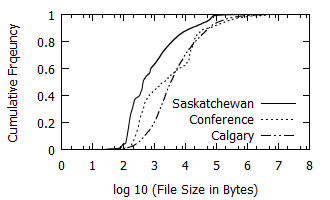
\includegraphics{images/filesize}
    \caption{Frequency of filesizes for files requested}\label{fig:filesize}
\end{figure}

\begin{table}
    \caption{Access Log Characteristics}\label{tab:characteristics}
    \begin{tabular}[ht!]{ | l || c | c | c | }
        \hline
        Invariant & Calgary & Saskatchewan & Conference \\
        \hline
        Success Rate & 96.07\% & 99.06\% & 96.78\% \\
        Mean Transfer & 10.9kB & 5.4kB & 23.0kB \\
        Median Transfer & 1697kB & 1712kB & 15015kB \\
        One Time Referencing & 32.4\% & 59.95\% & 43.27\% \\
        Cache Hit Rate & 13.5\% & 6.3\% & 16.3\% \\
        Cache Bytes Saved & 781MB & 525MB & 34.8GB \\
        Total Bytes Transferred & 7946MB & 13GB & 232GB \\
        \hline
    \end{tabular}
\end{table}

\begin{figure}[t]
    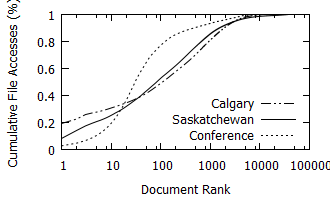
\includegraphics{images/concentration}
    \caption{Cumulative accesses to file vs file rank}\label{fig:file_accesses}
\end{figure}

\begin{figure*}
    \centering
    \begin{subfigure}{0.45\textwidth}
        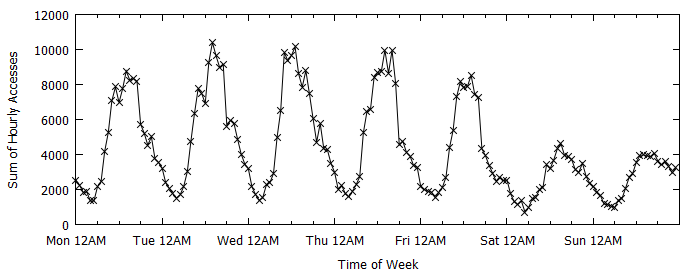
\includegraphics[width=\textwidth]{images/calgarytime}
        \caption{}\label{fig:calgary}
    \end{subfigure}
\qquad
    \begin{subfigure}{0.45\textwidth}
        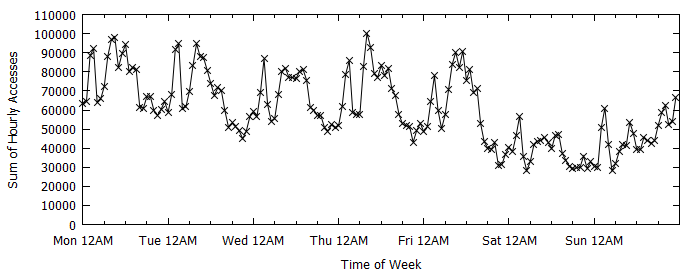
\includegraphics[width=\textwidth]{images/conferencetime}
        \caption{}\label{fig:conference}
    \end{subfigure}

    \begin{subfigure}{0.45\textwidth}
        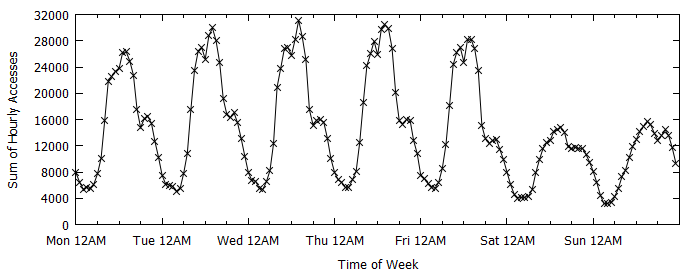
\includegraphics[width=\textwidth]{images/usasktime}
        \caption{}\label{fig:usask}
    \end{subfigure}
    \caption{Total file accesses grouped by hour of day for: (\ref{fig:calgary}) Calgary dataset, (\ref{fig:conference}) Conference dataset and (\ref{fig:usask}) dataset.) }\label{fig:diurnal}
\end{figure*}

\begin{figure*}
    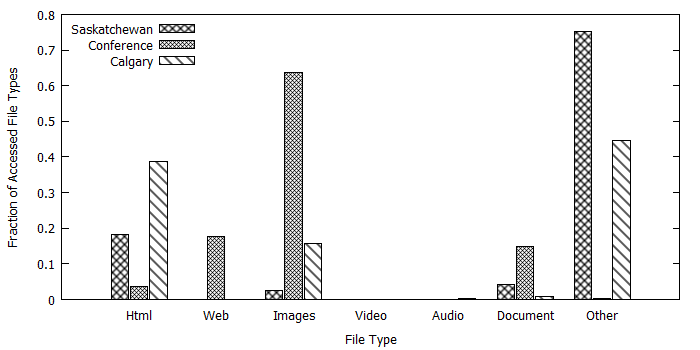
\includegraphics{images/filetype}
    \caption{Distribution of document types}\label{fig:file_types}
\end{figure*}

\subsection{Success Rate} % (fold)
\label{sub:success_rate}
For this invariant, we consider all 2XX and 3XX status code responses successful. This includes all of the successful, found, and not modified status codes that were examined separately on prior workload studies \cite{keynote, Faber}. The conference server log has a success rate very similar to that of Calgary’s department server log, and is 2.28\% lower than that of the University of Saskatchewan log. The success rate of the conference website strongly aligns with those from the original study by Arlitt and Williamson \cite{keynote}, and is an affirmation that the ability of web servers to respond to client requests have not changed and remain as reliable as they have been through the years. This observation may, however, only apply to academic websites as the average success rate between the four logs used in \cite{keynote, Faber} is 90.63\%. The scientific websites used in their study show a significantly higher failure rate, which suggest that the invariants may not hold true in the context of scientific sites.
% subsection success_rate (end)

\subsection{Document Types}\label{sub:doc_types}
We decided to analyse the number of times different file types were accessed and present these as a fraction of the total number of file accesses. We categorised files into HTML, images, web, video, audio, document and other. We defined the web category as files with the extensions \texttt{.css}, \texttt{.js}, \texttt{.cfm}, \texttt{.php}, \texttt{.asp}, \texttt{.aspx} and \texttt{.xml}. We also defined other as any files which were of an unknown type. We expected this to be useful characteristic to analyse as it allows us to see trends in what files are being accessed. The results of this analysis across all three Web servers are shown in Figure \ref{fig:file_types}.

The document type analysis revealed an interesting difference between the 2006-2007 log and the 1994-1995 logs. We can see that in the 1994-1995 logs, HTML was the most accessed document excluding documents of an unknown type. This observation is consistent with results obtained by Arlitt and Williamson \cite{keynote}. However, we can see that in the 2006-2007 log only a small fraction of the files accessed were HTML files. We can also note that in the 2006-2007 log, there were substantially more requests for images and Web file types than in the 1994-1995 logs. We have attributed this to increasing network bandwidth and advancements in the technology available for Web development.

\subsection{Concentration of References} % (fold)
\label{sub:concentration_of_references}
\begin{table}[h]
    \caption{The concentration of references of top 10\% distinct documents}\label{tab:conc_references}
    \begin{tabular}{l | l}
        Log & Accesses for top 10\% of documents\\
        \hline
        Calgary & 84.1\%\\
        Saskatchewan & 95.8\%\\
        Conference & 95.9\%
    \end{tabular}
\end{table}
Each server contains many different documents, and they certainly are not created equal; some files are in demand and some are rarely accessed. Users may demand certain files over others and access them at shorter intervals. Whereas other files are accessed rarely, if at all, thus accessed with longer intervals. We use concentration, a term which we use to define a non-uniform referencing behaviour, by first sorting the list of all distinct files by the number of times they were accessed in decreasing order. Afterwards, we plot the results using cumulative file accesses against the document ranking. Figure \ref{fig:file_accesses} shows the resulting plot for the three datasets.

Table \ref{tab:conc_references} shows that 10\% of all distinct documents were responsible for 84 - 96\% of requests received by servers in all the logs we analysed. The Conference dataset showed the most concentration and the other two datasets from Calgary and Saskatchewan showed similar but lower concentrations. Nevertheless all the data sets show similar trait in concentration of references. Another study by Mahanti et al.\cite{Mahanti} showed similar results and conclusion. This concentration aspect is another invariant of web workload characteristic in our server logs.
% subsection concentration_of_references (end)

\subsection{One Time Referencing} % (fold)
\label{sub:one_time_referencing}
The term one time referencing refers to the percentages of files that have only been requested once in a server log. In the original work by Arlitt and Williamson \cite{invariants} it was discovered that discovered that 23 - 42\% of the distinct files and 14 - 42\% of the distinct bytes were viewed only once in their datasets. They confirmed that approximately one third of the data were accessed only once, thus stating it as an invariant which has a great impact on the effectiveness of content caching.

Faber et al. \cite{Faber} conducted the same experiment ten years later. Their outcomes were significantly different where at least two-thirds of the files and bytes accessed in the log were accessed only once; 65 - 82\% of the files and 65 - 81\% of the bytes were requested only once in three of their servers. However, they did not completely disregard the original invariant because one of the access logs were of an academic institute compared to other three which were scientific Web servers.

Our results for one time referencing shows an outcome which lies in between the two studies \cite{invariants, Faber}. Figure \ref{tab:characteristics} shows that 32\% - 60\% of data files were accessed only once. The original invariant still holds true in these data sets, however the data set from University of Saskatchewan relates more to the latter study \cite{Faber}. Even though the two datasets are from universities, they display a notable differences. This suggests that results do not directly correlate to the type of server (i.e. server at a university and academic conference) but the presence of a dynamic content.

As stated in the study from \cite{invariants}, one time referencing is a concern. Depending on the server cache replacement policy, at least 30\% of the server cache are being wasted, thus proving server inefficiency.
% subsection one_time_referencing (end)

\subsection{File Size Distribution} % (fold)
\label{sub:file_size_distribution}
Figure \ref{fig:filesize} shows the file size distribution of the distinct files transferred by each site. As observed at the lower end of the graph for each server log, they all have a very few small files (less than 100 bytes). The majority of the files seem to be in the range of 100 - 100,000 bytes, while a few files are larger than 100,000 bytes. This file size distribution is consistent with results reported by other studies \cite{keynote, Braun}.

A trait we can see from the figure is that it is heavy-tailed. In other words, a heavy tail in a web file size distribution means that there are elephants, outliers, in the tail of the distribution. Although small in number, they are large enough to significantly affect the total traffic studied. The Pareto distribution \cite{Kotz}, can be observed in this file size distribution, for \begin{math} \alpha < 1\end{math}. The study by Crovella et al. \cite{Crovella} noted this observation and is confirmed in all three of our data sets.
% subsection file_size_distribution (end)

\subsection{Weekday vs Weekend} % (fold)
\label{sub:weekday_vs_weekend}
\begin{table}[h]
    \caption{Average weekday and weekend usage per day}\label{tab:weeklyusage}
    \begin{tabular}{l | c c}
        Log & Average Weekday Usage & Average Weekend Usage\\
        \hline
        Calgary & 119699 & 63207\\
        Saskatchewan & 387829 & 234720\\
        Conference & 1617134 & 1008210
    \end{tabular}
\end{table}

We examined the access time of our data sets and their trends throughout the week. The Calgary and Saskatchewan servers clearly show a dramatic decrease in average weekend access (63k) compared to weekday (120k), while the decrease on weekend traffic on the conference website-  was not nearly as significant. The percentage of weekend accesses at Saskatchewan are more similar to the percentage of conference website accesses than that of the Calgary site. Each of Calgary and Saskatchewan show a peak in weekday traffic around the middle of the week (Tuesday and Thursday respectively), while the conference website shows a drop from Monday to Wednesday, with the highest peak of the weekday on Thursday. Additionally, the conference website shows a positive trend on the weekend, starting from the lowest point of the week on Saturday, up to the regular weekday volume. We suspect that the increase in weekend traffic as a percentage of total traffic in the newest data set is due to computers and mobile devices being more readily available today.
% subsection weekday_vs_weekend (end)

\subsection{Daytime versus nighttime usage} % (fold)
\label{sub:daytime_versus_nighttime_usage}
Daytime versus nighttime usage in the Calgary and Saskatchewan servers are very different. Usage at night remains relatively the same throughout the week with the lowest points between 0:00 and 6:00. Daytime usage peaks between 12:00 and 15:00 each day, and form a platform around 18:00, after which usage drops steeply. This platform is seen more clearly on the Saskatchewan server than the Calgary server, and can be observed over the weekend on the Saskatchewan server. This observation is less obvious in the conference log. The conference log has an additional peak on each day of the week between 0:00 and 6:00 instead of a low which may be due to a global audience accessing the site. There is a no strong diurnal pattern in the weekdays with the lowest point just short of 0:00, and absolutely no diurnal pattern in the weekend, aligning with a previous study by Mahanti et al. \cite{Mahanti_Wu}. However there is clearly still a significant drop between 12:00 and 18:00 on each day between Monday and Saturday. 
% subsection daytime_versus_nighttime_usage (end)

\subsection{Caching} % (fold)
\label{sub:caching}
We looked at the HTTP status codes of requests within the three data sets and calculated the percentage of HTTP requests with a 304 (Not Modified) status code for each data set. We found the percentage of 304 status codes contribute 6.3\% of the total requests for the Saskatchewan data set, 13.5\% of the total requests for the Calgary data set, and 16.3\% of the total requests for the Conference data set. These results are summarised in the table \ref{tab:characteristics}.

Over the time period that each data set was logged, we calculated the total bytes saved by caching that the server didn’t need to transfer. This came to a total of 781MB of bandwidth saved from 7.9GB for the Calgary server, 525MB of bandwidth saved from 13GB for the Saskatchewan server and 34.8GB of bandwidth from 232GB for the conference server.

Data gathered about file caching on HTTP servers is useful as it can be applied to real world situations. By using this information to better understand how caching works on these types of servers, caching can be optimized to save bandwidth and resources for both the server and the requesting client.

% subsection caching (end)

\section{Discussion}\label{discussion}
Our analysis on document types revealed that in the conference Web server logs, approximately 65\% of requests were for images. This has practical uses as images are less likely to be changed than textual content. Therefore, there could be improvements made in caching architectures such that images have longer time to live values than other document types. This discovery aligns with a study by Gwertzman and Seltzer \cite{Gwertzman} which found that a conservative estimate for an image lifespan is 85-100 days. Additionally, due to the small size of images they are feasible to cache. As the percentage of requests for images has increased since the original study by Arlitt and Williamson \cite{invariants} as shown by figure \ref{fig:file_types}, the caching of images could greatly improve the performance of the Web.

\section{Conclusions and Future Work}\label{conclusions}

\bibliographystyle{IEEEtran}
\bibliography{references.bib}
\end{document}